\subsection{Physically Based Rendering}

In einer 3D-Szene eines Videospiels will man natürlich komplexere Objekte als simple Primitives darstellen. Diese Objekte bestehen aus vielen Primitives, in diesem Falle meist Dreiecke. 
Die Art der Zusammensetzung ist unterschiedlich. Manchmal kann es effizienter sein, aneinander hängende Dreiecke zu verwenden, jedoch werden meistens nur einzelne Dreiecke gerendert. 
Einige Programme verwenden %auch andere 
Polygone, welche aber auch aus Dreiecken bestehen. Daher ist dies irrelevant. 
Ein Objekt, gebildet aus Dreiecken, nennt man \textit{Mesh}. Als Beispiel ist das Mesh eines Delfins in \cref{Dolphin} dargestellt. Die Farbe bzw. die "`Haut"' eines Objektes wird aus einem zweidimensionalem Bild gelesen. Genannt wird dies \textit{Textur}.

\begin{figure}
	\begin{center}
		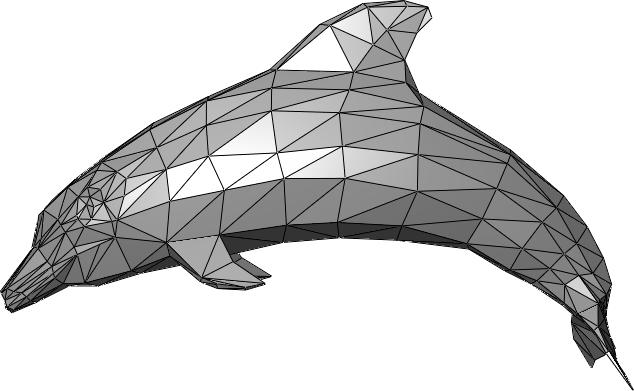
\includegraphics[width=0.5\textwidth]{06anhang/bilder/delphin.jpg}
		\caption{Mesh eines Delfins}
		\label{Dolphin}
	\end{center}
\end{figure}
 
Dafür besitzt jeder Vertex zusätzlich zu seiner Position eine zweidimensionale Position auf der Textur. So kann ermittelt werden, welche Pixel der Textur verwendet werden sollen.
Mit Mesh und Textur ist es möglich, ein Objekt in einer dreidimensionalen Szene anzuzeigen. In einem Videospiel würde dies jedoch nicht überzeugen. Es wird \ac{PBR} verwendet. \ac{PBR} ist eine Möglichkeit, eine realistischere dreidimensionale Szene zu erzeugen, indem physikalische Phänomene wie z.B. Licht berücksichtigt werden. 
Wie ein Objekt auf Licht reagiert, hängt von vier verschiedenen Größen ab: der eigentlichen Farbe des Objekts, der Oberflächenstruktur, der Farbe und der Richtung des einfallenden Lichts. Alle Eigenschaften eines Objekts, die sich auf die Farbe auswirken, werden in einem \textit{Material} zusammengefasst. 
Ein Objekt, welches gerendert werden soll, besitzt beides: 
ein \textit{Mesh} und ein \textit{Material}. Das ganze wird zusammengefasst \textit{Model} genannt.

Es gibt zwei Arten von Lichtquellen in der FM3D-Engine: \textit{Directional Light} und \textit{Point Lights}. Ein Directional Light besitzt eine Richtung, aber keine Position. Diese Art kann verwendet werden, um zum Beispiel eine Sonne zu simulieren, die so weit von der Erde entfernt ist, dass die Position irrelevant wird. Die Richtung der Strahlen hingegen ist wichtig und von der Tageszeit abhängig. 

Point Lights sind das genaue Gegenteil. Sie besitzen keine Lichtrichtung, sondern scheinen in alle Richtungen gleich. Dafür besitzen sie eine genau festgelegte Position, die relevant ist, da die Lichtstärke mit zunehmendem Abstand kleiner wird. Point Lights können verwendet werden, um die meisten Lichtquellen darzustellen (als Beispiel: Laternen oder Fackeln).

Man kann aber nicht nur zwischen Lichtquellen unterscheiden, sondern auch zwischen verschiedenen Arten des ausgesendeten Lichts. Die \ac{FM3D}-Engine verwendet ein Lichtmodell genannt "`Ambient/Diffuse/Specular"'. 
\textit{Ambient Light} ist das Licht, das man jeden Tag sieht, auch wenn gerade keine Sonne scheint oder man sich nicht in direkter Nähe einer Lichtquelle befindet. 
Es entsteht dadurch, dass Licht von allen Objekten wieder teilweise reflektiert wird und so eine schwache und gleichmäßige Beleuchtung entsteht. Ohne das Ambient Light wäre es hinter einem Haus, welches die Sonne verdeckt, komplett finster. 

Die zweite Lichtart ist \textit{Diffuse Light}, welches abhängig von dem Auftrittswinkel des Lichtstrahls ist. Betrachten wir einen Würfel, so sehen wir: 
die dem Licht zugewandte Seite ist heller, als die nur teilweise zugewandte Seite und die abgewandte Seite erfährt gar kein \textit{Diffuse Light}. 

\textit{Specular light} modelliert die Lichtstrahlen, welche von einem Objekt reflektiert und in die Linse der Kamera bzw. in die Augen des Betrachters gelangen. Dies wird als blendendes, helles Licht wahrgenommen und ist oft auf metallischen Oberflächen zu erkennen. Diese drei Lichtarten sind in \cref{Img:Lights} dargestellt.

Alle Lichtberechnungen müssen für jedes Pixel ausgeführt werden und laufen daher im Fragment-Shader ab.
Um die Farbe eines gerenderten Pixels zu bestimmen, benötigt man einige Informationen: die Position, die Farbe, den Normalenvektor und Specular-Factor des Pixels. Diese vier Informationen reichen für alle Lichtberechnungen aus. Die Phase, in der sie erstellt bzw. berechnet werden, ist unterschiedlich. Ein Teil wird außerhalb des Programms in externen Programmen erstellt und als Vertex im Mesh oder als Information im Material gespeichert. Dabei unterscheidet man zwischen:
\begin{itemize}
	\item Der Information, die sich für verschiedene Objekte unterscheidet, aber nicht innerhalb des Objekts
	\item Information, die für jeden Vertex anders ist aber für jeden Pixel nur linear interpoliert werden muss
	\item Information, die für jedes Pixel anders ist
\end{itemize}

Erstere kann einfach im Material gespeichert werden, da jedes Objekt ein eigenes Material haben kann und es anders als ein Mesh nicht viel Speicher benötigt. Die Vertexinformationen werden im \ac{VBO} des Mesh gespeichert und automatisch linear interpoliert, wenn sie an den Fragment-Shader weitergegeben werden. Pixelinformationen müssen einzeln in einer Textur gespeichert werden. Diese sind dann im Material enthalten, wobei diese nur referenziert werden, damit verschiedene Materials die gleichen Texturen verwenden können. In den Vertex-Informationen müssen hierfür zusätzlich Textur-Koordinaten gespeichert werden. Daraus ergeben sich die folgenden Werte, die in \cref{table:VertexAufbau} zu sehen sind.

Die FM3D-Engine verwendet \textit{Deferred Rendering}. Dies bedeutet, dass zuerst alle Objekte einer Szene gerendert und die Ergebnisse daraus in mehreren Buffern gespeichert werden, zusammengefasst \textit{G-Buffer} genannt. Danach wird für jede Lichtquelle ein weiterer Renderprozess ausgeführt, wobei die vorher genannten Buffer als Input dienen. Das Ergebnis ist in der \cref{Img:Lights} zu sehen. Der Vorteil hierbei ist, dass keine unnötige Lichtberechnungen ausgeführt werden muss, da alle Pixel später zu sehen sind und es keine Begrenzung für die Anzahl der Lichtquellen gibt. Der Aufbau des G-Buffers ist in \cref{table:GBuffer} zu sehen.

Im ersten Renderdurchgang wird nur in den G-Buffer die Informationen Position, Normalenvektor und Farbe des jeweiligen Fragments gespeichert. Der zweite Renderdurchgang ist abhängig von der Lichtquelle. Zusätzlich zum G-Buffer benötigt der Shader die Position der Kamera und die Farbinformationen der jeweiligen Lichtquelle. Die Farben für die drei Lichtarten werden dann nacheinander berechnet. Die Berechnung für Directional Light lautet folgendermaßen: 

Gegeben: \newline
	Lichtinformationen: Richtung: $\overrightarrow{r}$ Farbe: $\overrightarrow{L_{c}}$ Ambient und Diffuse Intensität: $L_{a}, L_{d}$ \newline
	GBufer: $\overrightarrow{G_{P}}, \overrightarrow{G_{N}}, \overrightarrow{G_{C}}$ \newline
	Kameraposition: $\overrightarrow{K}$ \newline
	Resultierende Farben der drei Lichtarten: $\overrightarrow{C_{A}},\overrightarrow{C_{D}},\overrightarrow{C_{S}}$\newline 
	Finale Farbe:  $\overrightarrow{C_{F}}$
	
	$\overrightarrow{C_{A}} = \overrightarrow{L_{c}} \cdot L_{a}$\newline
$\overrightarrow{C_{D}} = \overrightarrow{L_{c}} \cdot L_{d} \cdot (\overrightarrow{G_{N}} \cdot -\overrightarrow{r})$\newline
$\overrightarrow{x} = \overrightarrow{r} - 2 \cdot (\overrightarrow{G_{N}} \cdot \overrightarrow{r}) \cdot \overrightarrow{G_{N}}$\newline
$\overrightarrow{C_{S}} = \overrightarrow{L_{c}} \cdot \overrightarrow{G_{C alpha}} \cdot ((\overrightarrow{K} - \overrightarrow{G_{P}}) \cdot \overrightarrow{x})^{16}$
	
Die  Berechnung für ein Point Light ist gleich, nur ist die Farbe von der Position des Lichts abhängig und die Lichtrichtung von der Position des Fragments.

\begin{table}
	\caption{Vertex Aufbau}
	\label{table:VertexAufbau}
	\centering
	\begin{tabular}{lll}\toprule[1.5pt]
		Datentyp & Name & Beschreibung \\\midrule
		3D-Vektor & Position & Position des Vertex \\
		2D-Vektor & Textur Koordinate & Position des Vertex auf der Textur \\
		3D-Vektor & Normal & Normalenvektor zum Dreieck \\
		32-Bit Farbe & Color & Farbe des Vertex (optional, Standard ist weiß) \\
		3D-Vektor & Tangent & Tangentenvektor des Dreiecks. \\
		 & & Genaueres in \cref{section:Normalmapping}\\\bottomrule[1.5pt]
	\end{tabular}
	Quelle: Eigene Darstellung
\end{table}
\begin{table}
	\caption{Material Aufbau}
	\centering
	\begin{tabular}{lll}\toprule[1.5pt]
	Datentyp & Name & Beschreibung \\\midrule
	32-Bit Farbe & Color & Farbe des gesamten Objekts \\
	Textur & Color Texture & Gibt die Farbe jedes Pixels des Objektes an \\
	Textur & Normal map & Gibt den Normalenvektor jedes Pixels an. \\
	 & & Genaueres in \cref{section:Normalmapping} \\
	Float & Specular factor & Faktor für das resultierende Specular light \\
	Textur & Specular map & Specular factor für jeden Pixel. Der Faktor \\
	 & & des ganzen Objekts wird weiterhin verwendet \\
	 Boolean & UseWireframe & Gibt an ob ganze Dreiecke gerendert werden sollen\\
	  & & oder nur die Kanten. (Nützlich für Debugging)\\\bottomrule[1.5pt]
\end{tabular}
	Quelle: Eigene Darstellung
\end{table}

\begin{figure}
	\centering
	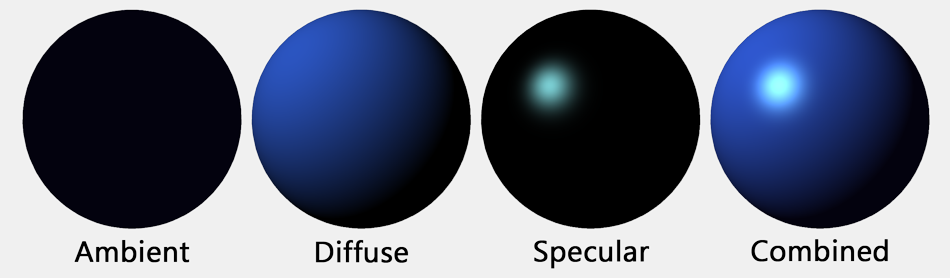
\includegraphics[scale=0.4]{02theorie/amb_diff_spec.png}
		
	Quelle: https://clara.io/img/pub/amb\textunderscore diff\textunderscore spec.png
	\caption{Lights}\label{Img:Lights}
\end{figure}

\begin{table}
	\caption{G-Buffer Aufbau}
	\label{table:GBuffer}
	\centering
	\begin{tabular}{rlll}\toprule[1.5pt]
		Größe & Name & Channels & Beschreibung \\\midrule
		96 Bit  & Position-Buffer & RGB mit je 32-Bit float & Position im Worldspace.\\
		128 Bit & Color-Buffer & RGBA mit je 32-Bit float & Farbe jedes Pixels in den Werten RGB und den Specular factor im Alpha-Wert \\
		96 Bit & Normal-Buffer & RGB mit je 32-Bit float & Normalenvektor im Worldspace \\
		32 Bit & Depth-Stencil-Buffer & 24 Bit Depth, 8 Bit Stencil & Depth- und Stencil-Wert des resultierenden Bildes \\
		128 Bit & Final-Buffer & RGBA mit je 32-Bit float & Resultierende Farbe jedes Pixels mit Alpha-Wert \\\bottomrule[1.5pt]
	\end{tabular}
\end{table}
